\documentclass[11pt,a4paper]{report}
%%%%%%%%%%%%%%%%%%%%%%%%%%%%%%%%%%%%%%%%%%%%%%%%%%%%%%%%%%%%%%%%%%%%%
%%                                                                 %%
%%    Header file for the Phi-S-X Series                           %%
%%                                                                 %%
%%    german version header_gm.tex is derived from header.tex      %%
%%    by uncommenting the line ``\setboolean{german}{true}'' below %%
%%                                                                 %%
%%    Never edit the german version! all changes must be done      %%
%%    in the english version header.tex                            %%
%%                                                                 %%
%%%%%%%%%%%%%%%%%%%%%%%%%%%%%%%%%%%%%%%%%%%%%%%%%%%%%%%%%%%%%%%%%%%%%
%%%%%%%%%%%%%%%%%%%%%%%%%%%%%%%%%%%%%%%%%%%%%%%%%%%%%%%%%%%%%%%%%%%%%
%%                                                                 %%
%%    Header file for the Phi-S-X Series                           %%
%%                                                                 %%
%%    german version header_gm.tex is derived from header.tex      %%
%%    by uncommenting the line ``\setboolean{german}{true}'' below %%
%%                                                                 %%
%%    Never edit the german version! all changes must be done      %%
%%    in the english version header.tex                            %%
%%                                                                 %%
%%%%%%%%%%%%%%%%%%%%%%%%%%%%%%%%%%%%%%%%%%%%%%%%%%%%%%%%%%%%%%%%%%%%%
%====================================================================
%-- define flag for language adaptations
\usepackage{ifthen}   % allows to select only certain text
\provideboolean{german}
\setboolean{german}{false}
%\setboolean{german}{true}  % uncomment this line for german editions
%====================================================================
%
% Textschriftart: Computer modern Bright
% body:            CM-Bright 10pt
% section titles:  CM-Bright Bold
% formulas:        CM-Bright Math Oblique
%
\usepackage[standard-baselineskips]{cmbright}
\usepackage{cmbright}
\usepackage[T1]{fontenc}
\def\usedfonts{CM-Bright}
\usepackage{typearea}
%\typearea[current]{calc} % benutzt die aktuelle 
       % bindekorrektur (BCOR angabe als parameter in koma usepackage)
       % und berechnet satzspiegel neu
\typearea[current]{11} %fixed div value

\usepackage{textcomp} % special symbols
\usepackage{amsfonts} % special symols
                      % see ftp://ftp.ams.org/pub/tex/doc/amsfonts/amsfndoc.pdf
\usepackage{amssymb}  % CM-Bright provides the AMS symbols
\usepackage{exscale}  % allows to scale math expressions to big fonts, 
                      % e.g. \Huge
\usepackage{curves}
\usepackage{braket}
\usepackage{miller}     % miller indices
\usepackage{chemmacros} % http://www.mychemistry.eu/mychemistry/
\usepackage[numbers]{natbib}     % bibliography style
\usepackage{url}\urlstyle{tt}
\usepackage{float}
\usepackage{bm}       % provides the command \bm{} that makes bold math symbols
\usepackage{amsmath}
\usepackage{amsbsy}   % allows bold mathematical symbols
\usepackage{amscd}
 \usepackage{a4wide}  % it is better to use the ``geometry'' package
\usepackage{array}    % 
\usepackage{fancyhdr} %  defines pagestyle fancy
\usepackage{epsfig}   % include graphics with epsfig
\usepackage{graphicx} % includegraphics
\usepackage{epstopdf}
\usepackage{wrapfig}
\usepackage{fancybox} % allows shadow-boxes
\usepackage{color}    % allows to use color in the text
%\usepackage{eepic}
\usepackage{flafter}  % places picture next to its reference
\usepackage{makeidx}  % make an index
%\usepackage{MnSymbol}  % 
%\usepackage{marvosym}  % 
\usepackage{textcase}
\usepackage{ulem} % defines strikeout \sout{}; underline \uline{}
                  % double underline \uuline{}; wave underline \uwave{}
                  % cross out \xout{}
%
%==========================================================================
%==  page layout  =========================================================
%==========================================================================
% eqnarray environment: reduce with of space in place of each ``&''
\setlength\arraycolsep{1.4pt}
\pagestyle{fancy}
%\renewcommand{\chaptermark}[1]{\markboth{\thechapter\ #1}{}}
\renewcommand{\chaptermark}[1]{\markboth{\MakeUppercase{\thechapter\ #1}}{}}
\fancyhf{} 
\fancyhead[LE]{\textsc{\thepage}\qquad\textsc{\leftmark}}
\fancyhead[RO]{\textsc{\leftmark}\qquad\textsc{\thepage}}
\renewcommand{\headrulewidth}{0.5pt}
\renewcommand{\footrulewidth}{0pt} 
\addtolength{\headheight}{2.5pt}
\fancypagestyle{plain}{\fancyhead{}
   \renewcommand{\headrulewidth}{0pt}
   \fancyfoot[CO]{\bfseries\thepage}}

% Line spacing -----------------------------------------------------------
\newlength{\defbaselineskip}
\setlength{\defbaselineskip}{\baselineskip}
\newcommand{\setlinespacing}[1]%
           {\setlength{\baselineskip}{#1 \defbaselineskip}}
\newcommand{\doublespacing}{\setlength{\baselineskip}%
                           {2.0 \defbaselineskip}}
\newcommand{\singlespacing}{\setlength{\baselineskip}{\defbaselineskip}}

% Absatz einr\"ucken ------------------------------------------------------
%\setlength{\parindent}{0pt}
\setlength{\parskip}{2pt}
% -------------------------------------------------------------------------
\ifthenelse{\boolean{german}}
  {\def\figurename{Abb.}}
  {\def\figurename{Fig.}}
%--------------------------------------------------------------------------
\renewcommand{\arraystretch}{1.15}  % skaliert den Zeilen abstand in der 
    % tabular und array umgebung
%
%==========================================================================
%==  boxes etc ============================================================
%==========================================================================
%== minipage in a shadowbox ===============================================
\newenvironment{myshadowminipage}[1]%
  {\par\noindent\begin{Sbox}\begin{minipage}{\linewidth}\vspace{0.1cm}\begin{center}\uppercase{#1}\end{center}}%
  {\vspace{0.1cm}\end{minipage}\end{Sbox}\shadowbox{\TheSbox}}
%
%== minipage in a framedbox ===============================================
\newenvironment{myframedminipage}%
  {\par\noindent\begin{Sbox}\begin{minipage}\linewidth\vspace{0.1cm}}%
  {\vspace{0.1cm}\end{minipage}\end{Sbox}\fbox{\TheSbox}}
%
\newcommand{\myshadowbox}[1]{\noindent\shadowbox{\parbox{\linewidth}{\smallskip #1\smallskip}}}
\newcommand{\myfbox}[1]{\noindent\fbox{\parbox{\linewidth}{\smallskip #1\smallskip}}\medskip}
%== minipage in a framedbox ===============================================
\newtheorem{defi}{Definition}[chapter]
\newenvironment{definition}[1]%
  {\par\noindent\begin{Sbox}\begin{minipage}{\linewidth}\vspace{0.1cm}\begin{defi}\uppercase{#1}\\\vspace{0.1cm}}%
  {\vspace{0.1cm}\end{defi}\end{minipage}\end{Sbox}\shadowbox{\TheSbox}}
%
%=========================================================================
% color used to point out information to the teacher
\definecolor{highlight}{rgb}{1.0,0.7,0.}
\newcommand{\Special}[1]{\textbf{\textcolor{highlight}{#1}}}
%=========================================================================
%  switch certain parts on and off. uses ifthen package
\newboolean{teacher}\setboolean{teacher}{false}
% this parameter can be changed in the manuscript again
\setboolean{teacher}{true} %private version if true!
\newcommand{\teacheronly}[1]{\ifthenelse{\boolean{teacher}}{#1\hfill\\ }}
\newcommand{\editor}[1]{\textcolor{blue}{\texttt{Editor: #1}}}
\newcommand{\MARK}[1]{\textcolor{blue}{#1}} 
\newcommand{\RED}[1]{\textcolor{red}{#1}} 
%
%==========================================================================
%==  define new symbols                                                 ===
%==========================================================================
% define \stat (stationary state) as an operator like \min
\DeclareMathOperator*{\stat}{stat}
\let\Vec=\mathbold   % cmbright.sty provides a bold/italic math alphabet
\let\Dot=\mathbold   % cmbright.sty provides a bold/italic math alphabet
\let\Ddot=\mathbold   % cmbright.sty provides a bold/italic math alphabet
%
\newcommand{\e}[1]{\mathrm{e}^{#1}}% exponential function
\renewcommand{\Re}{\mathrm{Re}}    % real part
\renewcommand{\Im}{\mathrm{Im}}    % imaginary part
\newcommand{\lagr}{\ell}           % Lagrange dichte
\newcommand{\Lagr}{\mathcal{L}}    % Lagrange Funktion
\newcommand{\erf}{{\rm erf}}       %
\newcommand{\atan}{{\rm atan}}     % arcus tangens
\newcommand{\mat}[1]{\bm{#1}}  % Matrix
\newcommand{\gmat}[1]{{\boldsymbol #1}}  % Matrix(symbol)
\newcommand{\defas}{\stackrel{\text{def}}{=}}  %  is defined as
\ifthenelse{\boolean{german}}
  {\newcommand{\rot}{{\rm\bf rot}}}    % curl
  {\newcommand{\rot}{{\rm\bf curl}}}   % curl
\newcommand{\sgn}{{\rm sgn}}       % sign
\ifthenelse{\boolean{german}}
   {\newcommand{\Tr}{\mathrm{Sp}}}      % trace
   {\newcommand{\Tr}{\mathrm{Tr}}}      % trace
\ifthenelse{\boolean{german}}
   {\newcommand{\grmn}[2]{\footnote{``#2'' hei{\ss}t in englisch ``#1''}}}
   {\newcommand{\grmn}[2]{\footnote{``#1'' translates as ``#2'' into German}}}
% define the equation reference
\ifthenelse{\boolean{german}}
   {\newcommand{\eq}[1]{\text{Gl.}~\ref{#1}}}
   {\newcommand{\eq}[1]{\text{Eq.}~\ref{#1}}}
% define a relation with an equation number ontop
\newcommand{\eqrel}[2]{\stackrel{\eq{#1}}{#2}}
\newcommand{\zero}{\varnothing}
%\newcommand{\ket}[1]{|#1\rangle} % contained in package braket
\newcommand{\sumint}{\int\hspace{-15pt}\sum}
\newcommand{\marker}[1]{\textcolor{blue}{\emph{#1}}}
\renewcommand*{\dot}[1]{\overset{\mbox{\large\bfseries .}}{#1}}
\renewcommand*{\ddot}[1]{\overset{\mbox{\large\bfseries\hspace{+0.1ex}.\hspace{-0.1ex}.}}{#1}}
%
%==========================================================================
%==                                                                     ===
%==========================================================================
% Prevent figures from appearing on a page by themselves
% from http://dcwww.camd.dtu.dk/~schiotz/comp/LatexTips/LatexTips.html
\renewcommand{\topfraction}{0.85}
\renewcommand{\textfraction}{0.1}
\renewcommand{\floatpagefraction}{0.75}
%
%==========================================================================
%==                                                                     ===
%==========================================================================
\makeindex    % make index. uses makeidx package.

%== allow links between documents ============================================
\usepackage{xr}
\usepackage{xr-hyper}
%==  hyperref package (must be last package)
\usepackage[colorlinks=true]{hyperref} %specify this as last package
\hypersetup{citecolor=blue}
\hypersetup{menucolor=magenta}
\hypersetup{urlcolor=blue}      % 
\hypersetup{filecolor=green}    % file links
\hypersetup{linkcolor=magenta}  %table of contents
\hypersetup{pdfauthor={Peter E. Bl\"ochl}}
\hypersetup{pdfdisplaydoctitle=true}
\externaldocument[phisx1-]{/Users/ptpb/Tree/PhiSX/ClassicalMechanics/Book/cm-gm}
\externaldocument[phisx2-]{/Users/ptpb/Tree/PhiSX/Electrodynamics/Book/el-gm}
\externaldocument[phisx3-]{/Users/ptpb/Tree/PhiSX/QuantumMechanics/Book/qm}
\externaldocument[phisx4-]{/Users/ptpb/Tree/PhiSX/StatisticalMechanics/Book/sm}
\externaldocument[phisxqm2-]{/Users/ptpb/Tree/PhiSX/QuantumMechanicsII/Book/qm2}
\externaldocument[phisxsm2-]{/Users/ptpb/Tree/PhiSX/StatisticalMechanicsII/Book/sm2}
\externaldocument[phisxcb-]{/Users/ptpb/Tree/PhiSX/Chemicalbond/Book/cb}
% Example: Figure~PhiSX:Quantum
% Mechanics-\ref{phisx3-fig:doubleslitwave} on page
% \pageref{phisx3-fig:doubleslitwave}


\hypersetup{pdftitle=paw_brillouin}
\begin{document}
\begin{titlepage}
\begin{center}
\vspace*{3.5cm}
{\huge \textbf{The Brillouin object of the CP-PAW code}}\\
\vspace{0.5cm}
{\large Peter E. Bl\"ochl}
\vspace{0.5cm} 
\end{center}

\vfill
\begin{center}
Copyright Peter E. Bl\"ochl; Sept.2, 2013-\today\\
{\small
Institute of Theoretical Physics;
Clausthal University of Technology;\\ 
D-38678 Clausthal Zellerfeld; Germany;\\
http://www.pt.tu-clausthal.de/atp/}
\end{center}
\end{titlepage}
\noindent            
\tableofcontents
%====================================================================
\chapter{BRILLOUIN object}
%====================================================================
%====================================================================
\section{Purpose and theoretical background}
%====================================================================
The purpose of this object is to perform integrations of matrix
elements over the occupied part of Brillouin zone.
\begin{eqnarray}
\langle A\rangle=\sum_n \frac{1}{V_G}\int d^3k\;
A_n(\vec{k})\theta(\epsilon_n(\vec{k})-\mu)
\end{eqnarray}
where the matrix of the one-particle operator $\hat{A}$ elements are
\begin{eqnarray}
A_n(\vec{k})=\langle\psi_n(\vec{k})|\hat{A}|\psi_n(\vec{k})\rangle
\end{eqnarray}
and $\epsilon_n(\vec{k})$ are the one-particle energies, the
eigenvalues of the Hamiltonian.

In the linear tetrahedron method\cite{jepsen71_ssc9_1763,
  lehmann72_pssb54_469, bloechl94_prb49_16223}, the function values
are evaluated at a set of discrete k-points $\vec{k}_j$ and energy
levels and matrix elements are linarly interpolated within tetrahedra
filling the space between the grid points.

The BRILLOUIN object selects the grid points and reduces them on the
basis of point groups symemtry operations of the crystal.

If the integral is performed as linear interpolation between grid
points, it can be written in the simple form
\begin{eqnarray}
\langle A\rangle=\sum_n\sum_{j} w_n(\vec{k}_j) A_n(\vec{k}_j)
\end{eqnarray}
where the integration weights are independent of the type if matrix
element to be integrated.\cite{bloechl94_prb49_16223} They are
evaluated using the tetrahedron method.

The integration weights include a quadratic correction, which improves
the integrals substantially beyond the purely linear
approximation.\cite{bloechl94_prb49_16223}

%================================================================
\section{Code structure: Brillouin}
%================================================================
%================================================================
\subsection{Brillouin\_module}
%================================================================
The object has an internal memory, which is kept in the Brillouin
module in the data structure \verb|THIS|.
\begin{verbatim}
TYPE THIS_TYPE
  INTEGER(4)             :: NKP       ! #(IRREDUCIBLE KPOINTS)
  INTEGER(4)             :: NTET      ! #(IRREDUCIBLE TETRAHEDRA)
  REAL(8)                :: VOL       ! 1/#(GENERAL TETRAHEDRA)
  REAL(8)                :: RBAS(3,3) ! REAL SPACE LATTICE VECTORS
  integer(4)             :: NKDIV(3)
  integer(4)             :: ishift(3)
  REAL(8)       ,POINTER :: XK(:,:)   !(3,NKP) IRR. K-POINTS IN RELATIVE COORDINATES
  INTEGER(4)    ,POINTER :: IKP(:,:)  !(4,NTET) TETRAHEDRON CORNERS
  INTEGER(4)    ,POINTER :: MULT(:)   !(NTET) MULTIPLICITY OF THE TETRAHEDRON
  INTEGER(4)    ,POINTER :: irrkp(:)  !(nmshp) pointer to irr. k-point
END TYPE THIS_TYPE
\end{verbatim}


%================================================================
\subsection{Brillouin\_msh}
%================================================================
\begin{itemize}
\item RBAS real-space lattice vectors in kartesian coordinates
\item NGKP Target value of the number of general
  k-points on the interpolation grid
\item NSYM number of generators for the point group operations 
\item IARB
\item TSHIFT
\end{itemize}

First, the k-point grid is defined by determining the division of the
lattice vectors $N(3)$ in \verb|brillouin_basdiv|. The value
$NMSHPNT=(N(1)+1)*(N(2)+1)*(N(3)+1)$ is returned. The grid divisions
are placed onto \verb|this%nkdiv|

In \verb|brillouin_reduz| the k-points are mapped onto each other
using the point group operations
\begin{eqnarray}
\vec{k}_{i_1,i_2,i_3}=\sum_{j=1}^3 \vec{g}_{j}\frac{i_{j}+\frac{1}{2}\tau_j}{n_{j}}
\nonumber
\vec{i}'=\mat{O}\vec{i}
\end{eqnarray}
In this way a mapping 
between k-points is established. For two symetry
related k-points the mapping always goes to the k-point with the lower
value according to some unique numbering scheme.

In \verb|brillouin_zuord| this mapping is used to determine the
irreducible k-points on the grid. The irreducible k-points are the
those that are mapped under the mapping \verb|NUM| onto themselfes
Those k-points will be calculated in relative coordinates as $XK$ an
the mapping $NUM$ will be modified so that the general k-points point
onto the irreducible k-points in their own arrangement.

The tetrahedra are calculated and mappend onto irreducible ones.

%====================================================================
\chapter{SPACEGROUP object}
%====================================================================
%====================================================================
\section{Purpose and theoretical background}
%====================================================================
%====================================================================
\subsection{Symmetry operations}
%====================================================================
The symmetry operations can be found in the book by Bradley and
Cracknell\cite{bradley72_book}, which lists in table~3.4
\textit{``Results of operatoes on the reciprocal lattice vectors''}
the point group operations in terms of reciprocal lattice vectors of
all the space-point groups of crystals. Note that the operations in
terms of real space lattice vectors differ from those in reciprocal
lattice vectors.

It is very important that the real-space lattice vectors are chosen
exactly in the convention of table~3.1 \textit{``The 14 Bravais
  lattices''} of Bradley Cracknell. There are different possible
choices, but only the one given in the book is compatible with teh
transformations in Table 3.4.

%====================================================================
\subsection{Bravais lattices}
%====================================================================
The SPACEGROUP object works only with the choice of unit cells used by
Bradley and Cracknell\cite{bradley72_book} in their table
\begin{center}
\begin{tabular}{|c|c|c|c|c|}
\hline
\multicolumn{2}{|c|}{Bravais Lattice} & $\vec{T}_1$& $\vec{T}_2$& $\vec{T}_3$\\
\hline
\hline
\multicolumn{5}{|c|}{triclinic}\\
\hline
primitive & $\Gamma_1$ & & &\\
\hline
%
\hline
\multicolumn{5}{|c|}{monoclinic}\\
\hline
primitive & $\Gamma_m$ & 
$(0,-b,0)$ & 
$(a\sin(\gamma),-a\cos(\gamma),0)$ 
&$(0,0,c)$ \\
base centered & $\Gamma_m^b$ & 
$(0,-b,0)$ & 
$\frac{1}{2}(a\sin(\gamma),-a\cos(\gamma),-c)$ &
$\frac{1}{2}(a\sin(\gamma),-a\cos(\gamma),c)$ \\
\hline
%
\hline
\hline
\multicolumn{5}{|c|}{orthorhombic}\\
\hline
primitive & $\Gamma_o$ & 
$(0,-b,0)$ & 
$(a,0,0)$ 
&$(0,0,c)$ \\
base centered & $\Gamma_o^b$ & 
$(\frac{1}{2}a,-\frac{1}{2}b,0)$ & 
$(\frac{1}{2}a,\frac{1}{2}b,0)$ & 
$(0,0,c)$ \\
body centered & $\Gamma_o^v$ & 
$\frac{1}{2}(a,b,c)$ & 
$\frac{1}{2}(-a,-b,c)$ & 
$\frac{1}{2}(a,-b,-c)$ \\
face centered & $\Gamma_o^f$ & 
$\frac{1}{2}(a,0,c)$ & 
$\frac{1}{2}(0,-b,c)$ & 
$\frac{1}{2}(a,-b,0)$ \\
\hline
%
\hline
\multicolumn{5}{|c|}{tetragonal}\\
\hline
primitive & $\Gamma_q$ & 
$(a,0,0)$ & 
$(0,a,0)$ 
&$(0,0,c)$ \\
\hline
body centered &$\Gamma_q^v$ & 
$\frac{1}{2}(-a,a,c)$ & 
$\frac{1}{2}(a,-a,c)$ & 
$\frac{1}{2}(a,a,-c)$ \\
\hline
%
\hline
\multicolumn{5}{|c|}{trigonal}\\
\hline
primitive & $\Gamma_{rh}$ & 
$(0,a,c)$ & 
$(\frac{1}{2}\sqrt{3}a,\frac{1}{2}a,c)$ &
$(-\frac{1}{2}\sqrt{3}a,\frac{1}{2}a,c)$ \\
\hline
%
\hline
\multicolumn{5}{|c|}{hexagonal}\\
\hline
primitive & $\Gamma_h$ & 
$(0,-1,0)a$ & 
$(\frac{1}{2}\sqrt{3},\frac{1}{2},0)a$ &
$(0,0,1)c$\\
\hline
%
\hline
\multicolumn{5}{|c|}{cubic}\\
\hline
primitive & $\Gamma_c$ & 
$(1,0,0)a$ & 
$(0,1,0)a$ & 
$(0,0,1)a$ \\
face centered & $\Gamma_c^f$ & 
$\frac{1}{2}a(0,1,1)$ & 
$\frac{1}{2}a(1,0,1)$ & 
$\frac{1}{2}a(1,1,0)$ \\
body centered & $\Gamma_c^v$ & 
$\frac{1}{2}a(-1,1,1)$ & 
$\frac{1}{2}a(1,-1,1)$ & 
$\frac{1}{2}a(1,1,-1)$ \\
\hline
\end{tabular}
\end{center}

%====================================================================
\subsection{Symmetry operations}
%====================================================================
\begin{center}
\begin{tabular}{|c|l|}
\hline
Schoenflies symbol &  Description\\
\hline
$E$ & identity \\
$I$ & inversion \\
$C_n$ & anticlockwise n-fold rotation (proper rotation)\\
$S_n$ & anticlockwise n-fold rotation\\
    & followed by a reflection about a plane \\
    & perpendicular to the rotation axis\\
$\sigma=C_2\cdot I$ & reflection\\
\hline
\end{tabular}
\end{center}
\begin{itemize}
\item The reflection can be expressed by a two-fold rotation about an axis
perpendicular to the mirror plane followed by an inversion.
%
\item The improper rotation $S(\phi)$ can also be expressed as product of a
proper rotation $C(\pi+\phi)$ followed by an inversion.
\begin{eqnarray}
C(\phi)&=&\left(\begin{array}{ccc}
\cos(\phi)& -\sin(\phi) & 0\\
\sin(\phi)& \cos(\phi) & 0\\
0& 0& 1\end{array}\right)
\qquad\;\qquad
S(\phi)=\left(\begin{array}{ccc}
\cos(\phi)& -\sin(\phi) & 0\\
\sin(\phi)& \cos(\phi) & 0\\
0& 0& -1\end{array}\right)
\nonumber\\
I\cdot C(\pi+\phi)
&=&\left(\begin{array}{ccc}
-\cos(\pi+\phi)& \sin(\pi+\phi) & 0\\
-\sin(\pi+\phi)& -\cos(\pi+\phi) & 0\\
0& 0& -1\end{array}\right)
=\left(\begin{array}{ccc}
-\cos(\pi+\phi)& \sin(\pi+\phi) & 0\\
-\sin(\pi+\phi)& -\cos(\pi+\phi) & 0\\
0& 0& -1\end{array}\right)
\nonumber\\
&=&\left(\begin{array}{ccc}
\cos(\phi)& -\sin(\phi) & 0\\
\sin(\phi)& \cos(\phi) & 0\\
0& 0& -1\end{array}\right)
=S(\phi)
\end{eqnarray}
Thus $S_3^+=I\cdot C_6^-$, $S_4^+=I\cdot C_4^-$ and $S_6^+=I\cdot C_3^-$. 
\end{itemize}


The following list explains all the symmetry elements for all lattice systems, and it contains a list of generators used lateron.
\begin{center}
\begin{tabular}{||c|c|||c|c||c|c||}
\hline
\multicolumn{6}{|c|}{Triclinic system $\Gamma_1$}\\
\hline
\multicolumn{6}{|c|}{Generators: $I, .... $}\\
\hline
\noalign{\medskip}
%
\hline
\multicolumn{6}{|c|}{Monoclinic system $\Gamma_m, \Gamma_m^b$}\\
\hline
2-fold rotation & axis &  & &  &\\
\hline
$C_{2z},\sigma_z$ & (1,0,0)  &  &  &   &\\  
\hline
\multicolumn{6}{|c|}{Generators: $I, .... $}\\
\hline
\noalign{\medskip}
%
\hline
\multicolumn{6}{|c|}{Orthorhomic system 
$\Gamma_o,\Gamma_o^b,\Gamma_o^v,\Gamma_0^f$}\\
%
\hline
2-fold rotation & axis &  & &  &\\
\hline
$C_{2x},\sigma_x$ & (1,0,0)  &  &  &   &\\  
$C_{2y},\sigma_y$ & (0,1,0)  &  &  &   &\\  
$C_{2z},\sigma_z$ & (0,0,1)  &  &  &   &\\  
\hline
\multicolumn{6}{|c|}{Generators: $I, .... $}\\
\hline
\noalign{\medskip}
%
\hline
\multicolumn{6}{|c|}{Tetragonal system $\Gamma_q,\Gamma_q^v$}\\
\hline
2-fold rotation & axis & 4-fold rotation &axis &  & \\
\hline
$C_{2x},\sigma_x$ & (1,0,0) &  $C^\pm_{4z},S^\mp_{4z}$ & (0,0,1) & & \\
$C_{2y},\sigma_y$ & (0,1,0) &  & & & \\
$C_{2z},\sigma_z$ & (0,0,1) &  & & & \\
$C_{2a},\sigma_a$ & (?,?,?) &  & & & \\
$C_{2b},\sigma_b$ & (?,?,?) &  & & & \\
\hline
\multicolumn{6}{|c|}{Generators: $I, .... $}\\
\hline
\noalign{\medskip}
%
\hline
\multicolumn{6}{|c|}{Trigonal system $\Gamma_{rh}$}\\
\hline
2-fold rotation & axis & 3-fold rotation &axis &  & \\
\hline
$C'_{21},\sigma_{d1}$ & (?,0,0)  & $C^\pm_3,S^\mp_6$ & (?,?,?) &   &\\  
$C'_{22},\sigma_{d2}$ & (?,0,0)  & &  &   &\\  
$C'_{23},\sigma_{d3}$ & (?,0,0)  & &  &   &\\  
\hline
\multicolumn{6}{|c|}{Generators: $I, .... $}\\
\hline
\noalign{\medskip}
%
\hline
\multicolumn{6}{|c|}{Hexagonal system $\Gamma_h$}\\
\hline
2-fold rotation & axis & 3-fold rotation &axis &6-fold rotation  & axis\\
\hline
$C_{2},\sigma_h$ & (?,?,?)  & $C^\pm_3,S^{\mp}_6$ & (?,?,?)  & $C^{\pm}_6,S^{\mp}_3$  & (?,?,?)\\  
$C'_{21},\sigma_{d1}$ & (?,?,?)  &  &  &   &\\  
$C'_{22},\sigma_{d2}$ & (?,?,?)  &  &  &   &\\  
$C'_{23},\sigma_{d3}$ & (?,?,?)  &  &  &   &\\  
$C''_{21},\sigma_{v1}$ & (?,?,?)  &  &  &   &\\  
$C''_{22},\sigma_{v2}$ & (?,?,?)  &  &  &   &\\  
$C''_{23},\sigma_{v3}$ & (?,?,?)  &  &  &   &\\  
\hline
\multicolumn{6}{|c|}{Generators: $I, .... $}\\
\hline
\end{tabular}
\end{center}
\begin{center}
\begin{tabular}{||c|c|||c|c||c|c||}
\hline
\multicolumn{6}{|c|}{Cubic system $\Gamma_c,\Gamma_c^f,\Gamma_c^v$
(see Fig. 1.3 of Bradley Cracknell\cite{bradley72_book})}\\
\hline
2-fold rotation & axis & 3-fold rotation & axis &4-fold rotation & axis \\
\hline
$C_{2x},\sigma_x$ & (1,0,0)  & $C_{31}$ & (1,1,1)  &   $C_{4x}$ & (1,0,0)\\  
$C_{2y},\sigma_y$ & (0,1,0)  & $C_{32}$ & (-1,-1,1)&   $C_{4y}$ & (0,1,0)\\  
$C_{2z},\sigma_z$ & (0,0,1)  & $C_{33}$ & (1,-1,-1)&   $C_{4z}$ & (0,0,1)\\  
$C_{2a},\sigma_a$ & (1,1,0)  & $C_{34}$ & (-1,1,-1)&           &\\  
$C_{2b},\sigma_b$ & (1,-1,0) &         &    & &\\
$C_{2c},\sigma_c$ & (1,0,1)  &         &  & &\\
$C_{2d},\sigma_d$ & (0,1,1)  &         &  & &\\
$C_{2e},\sigma_e$ & (0,1,1)  &         &  & &\\
$C_{2f},\sigma_f$ & (0,-1,1) &         &  & &\\
\hline
\multicolumn{6}{|c|}{Generators: $I, C_{2x}, C_{2z}, C_{2a}, \sigma_{da}, C^+_{31}$}\\
\hline
\end{tabular}
\end{center}
A supersript on the Bravais-lattice symbol $\Gamma$ means
base-centered (b), body-centered (v), face-centered (f). The primitive
lattice has no superscript.

All lattice systems can have the identity $E$ and the inversion $I$ as
one of its symmetry elements. They are not listed.


%% Symmetry symbols according to table 1.2 of Bradley Cracknell.
%% \begin{center}
%% \begin{tabular}{|c|c|l|}
%% \hline
%% Schoenflies symbol & parameters. & Description\\
%% \hline
%% $E$       & E    & identity   \\
%% $I=-E$    & INV  & inversion  \\
%% \hline
%% $C_{2}$   & & \\
%% $C_{2j}$  & j=x,y,z,a,b,v,d,e,f& \\
%% $C'_{2j}$ & j=1,2,3 &\\
%% $C''_{2j}$ & j=1,2,3 &\\
%% \hline
%% $\sigma_{h}=I\cdot C_2$ & & \\
%% $\sigma_{j}=I\cdot C_{2j}$ & j=x,y,z,a,b,v,d,e,f& \\
%% $\sigma_{dj}$ & j=1,2,3,a,b,c,d,e,f& \\
%% $\sigma_{vj}$  & j=1,2,3& \\
%% \hline
%% $C_3^\pm$ & $\pm=+,-$ & \\
%% $C_{3j}^\pm$ & $j=1,2,3,4; \pm=+,-$ & \\
%% \hline
%% $S_3^\pm=I\cdot C_6^\mp$ & $\pm=+,-$ \\
%% $S_{3j}^\pm=I\cdot C_{lj}^\mp$   & $j=1,2,3,4; \pm=+,-$ & \\
%% \hline
%% $C_{4j}^\pm$ & $j=x,y,z; \pm=+,-$ & \\
%% $S_{4j}^\pm$ & $j=x,y,z; \pm=+,-$ & \\
%% \hline
%% $C_6^\pm$ & $\pm=+,-$ & \\
%% $C_{6j}^\pm$ & $j=1,2,3,4; \pm=+,-$ &\\
%% \hline
%% $S_6^\pm$ & $\pm=+,-$ & \\
%% $S_{6j}^\pm$ & $j=1,2,3,4; \pm=+,-$ & \\
%% \hline
%% \end{tabular}
%% \end{center}


%% \begin{center}
%% \begin{tabular}{|c|c|l|}
%% \hline
%% Schoenflies symbol & Internal repr. & Description\\
%% \hline
%% $C_2$ & & \\
%% $C_{2x}$   & C2X  & two-fold rotation about x-axis\\
%% $C_{2y}$   & C2Y  & two-fold rotation about y-axis \\
%% $C_{2z}$   & C2Z  &two-fold rotation about z-axis \\
%% $C_{2a}$    & C2A & two-fold rotation about the ?? axis\\ 
%% $C_{2b}$    & C2B & two-fold rotation about the ?? axis\\ 
%% $C'_{21}$ & c21s & \\
%% $C'_{22}$ & c21s & \\
%% $C'_{23}$ & c21s & \\
%% $C''_{21}$ & & \\
%% $C''_{22}$ & & \\
%% $C''_{23}$ & & \\
%% \hline
%% $\sigma_{d1}$ & & \\
%% $\sigma_{d2}$ & & \\
%% $\sigma_{d3}$ & & \\
%% $\sigma_h$ & & \\
%% $\sigma_{v1}$& & reflection\\
%% $\sigma_{v2}$& & reflection\\
%% $\sigma_{v3}$& & reflection\\
%% $\sigma_x=-C_{2x}$ & -C2X &  reflection at yz plane\\
%% $\sigma_y=-C_{2y}$ & -C2Y & reflection at xz plane \\
%% $\sigma_z=-C_{2z}$ & -C2Z & reflection at xy plane\\
%% $\sigma_{da}$ & -C2A? &  reflection about the ?? plane\\
%% $\sigma_{db}$ & -C2B?&  reflection about the ?? plane\\
%% \hline
%% $C_{3}^+ $  & C3P & 120$^\circ$ rotation about the c-axis\\
%% $C_{3}^- $  & C3M & -120$^\circ$ rotation about the c-axis\\
%% $C_{31}^+ $ & C31P & 120$^\circ$ rotation about the ?? axis\\
%% $C_{32}^+ $ & C31P & 120$^\circ$ rotation about the ?? axis\\
%% $C_{33}^+ $ & C31P & 120$^\circ$ rotation about the ?? axis\\
%% $C_{34}^+ $ & C31P & 120$^\circ$ rotation about the ?? axis\\
%% \hline
%% $S_{3}^+ $ & -C3M &  \\
%% $S_{3}^- $ & C3M  &  \\
%% \hline
%% $C_{4z}^+$  & C4ZP & rotation by +90 degree about the z axis\\
%% $C_{4z}^-$  & C4ZM &  rotation by -90 degree about the z axis \\
%% \hline
%% $S_{4z}^+=-C_{4z}^-$ &-C4ZM &  rotation by 90 degree about the z axis\\
%%             & &       followed by reflection at the xy plane.\\
%% $S_{4z}^-=-C_{4z}^+$ &-C4ZP &  rotation by 90 degree about the z axis\\
%%             & &       followed by reflection at the xy plane.\\
%% \hline
%% $C_{6}^+ $ & C6P & 60$^\circ$ rotation about the c-axis\\
%% $C_{6}^- $ & C6M & -60$^\circ$ rotation about the c-axis\\
%% $S_{6}^+ $ & -C6M  &  \\
%% $S_{6}^- $ &  C6M  &  \\
%% \hline
%% \end{tabular}
%% \end{center}

%====================================================================
\subsection{Symmetry operations: Table 3.4 of Bradley Cracknell}
%====================================================================
The transformations are converted into matrices as follows: Let us
take the operation $C^+_{32}$ for the face-centered cubic lattice
$\Gamma^f_c$:
\begin{table}[h!]
\begin{center}
\begin{tabular}{|l|c|c|c|}
\hline
&\multicolumn{3}{|c|}{$\Gamma^f_c$}\\
\hline
$C^+_{32}$ & $-\vec{g}_1-\vec{g}_2-\vec{g}_3$ & $\vec{g}_1$ & $\vec{g}_3$\\
\hline
\end{tabular}
\end{center}
\caption{\label{tab:explanationbradleytable34} Example for an entry of
  table 3.4 of Bradley Cracknell\cite{bradley72_book}}
\end{table}

The three entries in table~\ref{tab:explanationbradleytable34} specify
the result of the operation $C^+_{32}$ onto the first, second, and
third lattice vector, that is
$\vec{g}'_1=\mat{U}^{C^+_{32}}\vec{g}_1$,
$\vec{g}'_2=\mat{U}^{C^+_{32}}\vec{g}_2$ and
$\vec{g}'_3=\mat{U}^{C^+_{32}}\vec{g}_3$. Here, $\mat{U}^{C^+_{32}}$
is the transformation in cartesian coordinates, and $\vec{g}_i$ are
the primitive reciprocal lattice vectors in cartesian coordinates.


The transformation $C^+_{32}$ can be written as sum of dyadic products
\footnote{Dyadic products (outer products) of two vectors are written
  as $\vec{a}\otimes\vec{b}$. The resulting matrix gas the elements
  $(\vec{a}\otimes\vec{b})_{i,j}=a_ib_j$}
\begin{eqnarray}
\mat{U}^{C^+_{32}}&=&
(-\vec{g}_1-\vec{g}_2-\vec{g}_3)\otimes\vec{g}_1
+\vec{g}_1\otimes\vec{g}_2
+\vec{g}_3\otimes\vec{g}_3
=\sum_{i,j}O^{\Gamma^f_c,C^+_{32}}_{i,j}  \vec{g}_i\otimes\vec{g}_j
\end{eqnarray}
The matrix 
\begin{eqnarray}
\mat{O}^{\Gamma^f_c,C^+_{32}} =
\left(\begin{array}{ccc}
-1 & 1 & 0 \\
-1 & 0 & 0 \\
-1 & 0 & 1\\
\end{array}\right)
\label{eq:Oex}
\end{eqnarray}
is the transformation $C^+_{32}$ expressed in relative coordinates of
the reciprocal lattice vectors $\vec{g}_1,\vec{g}_2,\vec{g}_3$
specified in Table 3.3 of Bradley Cracknell\cite{bradley72_book} for
the face-centered cubic Bravais system $\Gamma^f_c$.  The matrices
$\mat{O}$ can be obtained directly from table~3.4 of Bradley
Cracknell\cite{bradley72_book}.

The meaning of $\mat{O}^{\Gamma^f_c,C^+_{32}}$ as defined in
\eq{eq:Oex} is the following: Under the transformation $C^+_{32}$, the
first reciprocal lattice vector $\vec{g}_1$ is transformed onto
$\vec{g}_1'=-\vec{g}_1-\vec{g}_2-\vec{g}_3$, the second on
$\vec{g}'_2=\vec{g}_1$ and that the third vector remains unchanged,
i.e. $\vec{g}'_3=\vec{g}_3$.

Note, that the choice made in Table 3.3 of Bradley Cracknell is not
unique. The form of the matrix $\mat{O}^{\Gamma^f_c,C^+_{32}}$ relies on the choice of lattice vectors made by Bradley and Cracknell.

The reciprocal lattice vectors can be combined into the matrix
$\mat{g}$. For the example given above, the matrix $\mat{g}$ has,
according to table 3.3, the form
\begin{eqnarray}
\mat{g}^{\Gamma^f_c}=(\vec{g}_1,\vec{g}_2,\vec{g}_3)=\frac{2\pi}{a}
\left(
\begin{array}{rrr}
-1 & 1& 1\\
 1 & -1& 1\\
 1 & 1& -1 \\
\end{array}\right)
\label{eq:matrixgforgfc}
\end{eqnarray}

The matrix $\mat{g}$ transforms a point $\vec{G}$ in reciprocal space
from the relative coordinates $\vec{x}$ into cartesian (absolute)
coordinates $\vec{G}$, i.e. $\vec{G}=\mat{g}\vec{x}$.  Thus, a
transformation can be written in relative and absolute coordinates as
\begin{eqnarray}
\vec{G}'=\mat{U}\vec{G}
\nonumber\\
\vec{x'}=\mat{O}\vec{x}
\end{eqnarray}

Thus, the operation $\mat{U}$ in Cartesian coordinates is obtained from
$\mat{O}$
\begin{eqnarray}
\mat{U}=\mat{g}\mat{O}\mat{g}^{-1}
\label{eqLfromotiuing}
\end{eqnarray}

For the specific example, we obtain
\begin{eqnarray}
\mat{U}^{C^+_{32}}&=&\mat{g}^{\Gamma^f_c}\mat{O}^{\Gamma^f_c,C^+_{32}}
\left(\mat{g}^{\Gamma^f_c}\right)^{-1}
=
\underbrace{\frac{2\pi}{a}\left(\begin{array}{rrr}
-1 & 1& 1\\
 1 & -1& 1\\
 1 & 1& -1 \\
\end{array}\right)}_{\mat{g}}
\underbrace{\left(\begin{array}{ccc}
-1 & 1 & 0 \\
-1 & 0 & 0 \\
-1 & 0 & 1\\
\end{array}\right)}_{\mat{O}}
\underbrace{\frac{a}{2\pi}\cdot\frac{1}{2}
\left(\begin{array}{rrr}
0 & 1& 1\\
 1 & 0& 1\\
 1 & 1& 0 \\
\end{array}\right)}_{\mat{g}^{-1}}
\nonumber\\
&=&\left(\begin{array}{rrr}
 0 &  0& -1\\
 1 &  0&  0\\
 0 & -1&  0 \\
\end{array}\right)
\end{eqnarray}
The result is a three fold rotation about the axis $(1,1,-1)$
expressed in cartesian coordinates, while
$\mat{O}^{\Gamma^f_c,C^+_{32}}$ is the same operation expressed in
relative coordinates for the lattice vectors $\mat{g}^{\Gamma^f_c}$.

%====================================================================
\subsection{Transformation matrices}
%====================================================================
Because the Brillouin object transforms the points on the grid, it
directly works with relative coordinates $\vec{x}$. A k-point is given as
\begin{eqnarray}
\vec{G}_{i_1,i_2,i_3}=\mat{g}\vec{x}_{i_1,i_2,i_3}
\end{eqnarray}
where
$\vec{x}_{i_1,i_2,i_3}=(\frac{i_1-1}{n_1},\frac{i_2-1}{n_2},\frac{i_3-1}{n_3})$
and therefore $\vec{k}_{i_1,i_2,i_3}= \vec{g}_1
\frac{i_1-1}{n_1}+\vec{g}_2 \frac{i_2-1}{n_2} +\vec{g}_3\frac{i_3-1}{n_3}$.
In order to transform the indices $(i_1,i_2,i_3)$, we only need the
matrix $\mat{O}$.

The operations needed by the Brillouin object are these matrices
$\mat{O}$

%====================================================================
\subsubsection{Convert operations from reciprocal to real space}
%====================================================================
If the operations $\mat{O}$ are given for reciprocal space, the ones
in real space can be constructed via a transformation into cartesian
coordinates.

Let $\mat{O}$ be the operation relative to the reciprocal lattice
vectors $\mat{g}$, and $\mat{P}$ the operation relative to the real
lattice vectors $\mat{T}$. We obtain the conversion by
\begin{eqnarray}
\mat{U}&\eqrel{eqLfromotiuing}{=}&\mat{g}\mat{O}\mat{g}^{-1}
\nonumber\\
\mat{U}&=&\mat{T}\mat{P}\mat{T}^{-1}
\nonumber\\
\Rightarrow
\mat{P}
&=&\mat{T}^{-1}\mat{g}\mat{O}\mat{g}^{-1}\mat{T}
=\mat{T}^{-1}\Bigl(2\pi\mat{T}^{-1,\top}\Bigr)
\mat{O}\Bigl(2\pi\mat{T}^{-1,\top}\Bigr)^{-1}\mat{T}
\nonumber\\
&=&\mat{T}^{-1}\mat{T}^{-1,\top}
\mat{O}\mat{T}^{\top}\mat{T}
\nonumber\\ 
&=&\Bigl(\mat{T}^{\top}\mat{T}\Bigr)^{-1}
\mat{O}\Bigl(\mat{T}^{\top}\mat{T}\Bigr)
\label{eq:oppfromo}
\end{eqnarray}

If the matrix $\mat{P}$ contains non-integer entries, there is an
inconsistency between the operations and the Bravais lattice chosen.




%====================================================================
\subsection{Generators}
%====================================================================
The point group can be built up from a small number of generators.
All operations in a point group can be obtained from the set of
generators by multiplying the generators in arbitrary combinations
and powers with each other. 

The generators for each of the 230 point groups are listed in
table~3.7 of Bradley Cracknell. We observe that there are at most five
generators for each point group.


%================================================================
\section{Code structure: Spacegroup}
%================================================================
It is important to initialize the spacegroup object by specifying a
space group. This is done by giving the space group number using
\verb|SPACEGROUP$SETI4('spacegroup',VAL)|. All subsequent operations
will refer to this spacegroup only. Changing to a different space
group is possible at any time.

The subroutines are
\begin{verbatim}
SUBROUTINE SPACEGROUP$SETI4(ID,VAL)
SUBROUTINE SPACEGROUP$GETCH(ID,VAL)
SUBROUTINE SPACEGROUP$RBAS(BRAVAIS,A0,B0,C0,ALPHA,BETA,GAMMA,RBAS)
  SUBROUTINE SPACEGROUP$ABCALPHABETAGAMMA(SWITCH,A,B,C,ALPHA,BETA,GAMMA,T)
SUBROUTINE SPACEGROUP$GENERATORS(ID,NOPX,NOP,OPERATION,C)
SUBROUTINE SPACEGROUP$COMPLETE(NOPX,NOP,OP,C)
\end{verbatim}

\begin{itemize}
\item with \verb|SPACEGROUP$SETI4('SPACEGROUP',val)| one sets the
  spacegroup by its space group number
%
\item with \verb|SPACEGROUP$GETCH('BRAVAIS',val)| one retrieves the
  symbol for the corresponding bravais lattice
%
\item with \verb|SPACEGROUP$RBAS| one specifies the lattice vectors by
  supplying the lattice parameters $a,b,c,\alpha,\beta,\gamma$. Note
  that angles are given in radian (not degree).
%
\item with \verb|SPACEGROUP$GENERATORS| the generators of the group
  are obtained either in real or in reciprocal space.
%
\item with \verb|SPACEGROUP$COMPLETE| the set of generators is
  expanded to the full point group.
\end{itemize}


%================================================================
\subsection{SPACEGROUP\$GENERATORS}
%================================================================
With \verb|ID='REAL'| or \verb|ID='RECI'| one selects the operations
in real or reciprocal space. Note that the translations \verb|C| are
zero in reciprocal space.

An operation is specified by an integer matrix $\mat{O}$, which
transforms the reciprocal lattice vectors and a vector $\vec{c}$ which
defines the transformation of the relative coordinates in real space
as
\begin{eqnarray}
\vec{x'}=\mat{P}\vec{x}+\vec{c}
\end{eqnarray}
The cartesian coordimates are then
\begin{eqnarray}
\vec{r'}=\mat{T}\mat{P}\mat{T}^{-1}\vec{r}+\mat{T}\vec{c}
\end{eqnarray}
where $\mat{T}$ is the matrix of real-space lattice vectors.

The real space operation $\mat{P}$ is obtained from the reciprocal
space operation $\mat{O}$ via \eq{eq:oppfromo}.

%================================================================
%\subsection{SPACEGROUP\$GENERATORS}
%================================================================


\appendix
%====================================================================
\newpage
\section{Spacegroups}
%====================================================================
The translation between the spacegroup number and the international
space group symbols is given in tables~\ref{table:spacegroupnumber_a}
and \ref{table:spacegroupnumber_b}.
\begin{table}[h!]
\begin{center}
\begin{tabular}{||r|l||r|l||r|l||r|l||r|l||}
\hline
1      & P1                 & 
2      & P$\bar{1}$         & 
3      & P2                 & 
4      & P2$_1$             & 
5      & C2                 \\
6      & Pm                 & 
7      & Pc                 & 
8      & Cm                 & 
9      & Cc                 & 
10     & P2/m               \\
11     & P2$_1$/m           & 
12     & C2/m               & 
13     & P2/c               & 
14     & P2$_1$/c           & 
15     & C2/c               \\
16     & P222               & 
17     & P222$_1$           & 
18     & P2$_1$2$_1$2       & 
19     & P2$_1$2$_1$2$_1$   & 
20     & C222$_1$           \\
21     & C222               & 
22     & F222               & 
23     & I222               & 
24     & I2$_1$2$_1$2$_1$   & 
25     & Pmm2               \\
26     & Pmc2$_1$           & 
27     & Pcc2               & 
28     & Pma2               & 
29     & Pca2$_1$           & 
30     & Pnc2               \\
31     & Pmn2$_1$           & 
32     & Pba2               & 
33     & Pna2$_1$           & 
34     & Pnn2               & 
35     & Cmm2               \\
36     & Cmc2$_1$           & 
37     & Ccc2               & 
38     & Amm2               & 
39     & Aem2               & 
40     & Ama2               \\
41     & Aea2               & 
42     & Fmm2               & 
43     & Fdd2               & 
44     & Imm2               & 
45     & Iba2               \\
46     & Ima2               & 
47     & Pmmm               & 
48     & Pnnn               & 
49     & Pccm               & 
50     & Pban               \\
51     & Pmma               & 
52     & Pnna               & 
53     & Pmna               & 
54     & Pcca               & 
55     & Pbam               \\
56     & Pccn               & 
57     & Pbcm               & 
58     & Pnnm               & 
59     & Pmmn               & 
60     & Pbcn               \\
61     & Pbca               & 
62     & Pnma               & 
63     & Cmcm               & 
64     & Cmce               & 
65     & Cmmm               \\
66     & Cccm               & 
67     & Cmme               & 
68     & Ccce               & 
69     & Fmmm               & 
70     & Fddd               \\
71     & Immm               & 
72     & Ibam               & 
73     & Ibca               & 
74     & Imma               & 
75     & P4                 \\
76     & P4$_1$             & 
77     & P4$_2$             & 
78     & P4$_3$             & 
79     & I4                 & 
80     & I4$_1$             \\
81     & P$\bar{4}$                & 
82     & I$\bar{4}$                & 
83     & P4/m               & 
84     & P4$_2$/m           & 
85     & P4/n               \\
86     & P4$_2$/n           & 
87     & I4/m               & 
88     & I4$_1$/a           & 
89     & P422               & 
90     & P42$_1$2           \\
91     & P4$_1$22           & 
92     & P4$_1$2$_1$2       & 
93     & P4$_2$22           & 
94     & P4$_2$2$_1$2       & 
95     & P4$_3$22           \\
96     & P4$_3$2$_1$2       & 
97     & I422               & 
98     & I4$_1$22           & 
99     & P4mm               & 
100    & P4bm               \\
101    & P4$_2$cm           & 
102    & P4$_2$nm           & 
103    & P4cc               & 
104    & P4nc               & 
105    & P4$_2$mc           \\
106    & P4$_2$bc           & 
107    & I4mm               & 
108    & I4cm               & 
109    & I4$_1$md           & 
110    & I4$_1$cd           \\
111    & P$\bar{4}$2m              & 
112    & P$\bar{4}$2c              & 
113    & P$\bar{4}$2$_1$m          & 
114    & P$\bar{4}$2$_1$c          & 
115    & P$\bar{4}$m2              \\
116    & P$\bar{4}$c2              & 
117    & P$\bar{4}$b2              & 
118    & P$\bar{4}$n2              & 
119    & I$\bar{4}$m2              & 
120    & I$\bar{4}$c2              \\
\hline
\end{tabular}
\end{center}
\caption{\label{table:spacegroupnumber_a}Space group number as given
  in the ``International tables for Crystallography, Vol. A'' and the
  corresponding international space group symbol (Herman-Maughin
  notation). Retrieved from the Bilbao Crystallographic Server
  \url{http://www.cryst.ehu.es/cryst/text/table.html} on Dec. 21,
  2013.  For further information, see Aroyo, et. al. Zeitschrift f\"ur
  Kristallographie (2006), 221, 1, 15-27.  }
\end{table}


\begin{table}[H]
\begin{center}
\begin{tabular}{||r|l||r|l||r|l||r|l||r|l||}
\hline
121    & I$\bar{4}$2m              & 
122    & I$\bar{4}$2d              & 
123    & P4/mmm             & 
124    & P4/mcc             & 
125    & P4/nbm             \\
126    & P4/nnc             & 
127    & P4/mbm             & 
128    & P4/mnc             & 
129    & P4/nmm             & 
130    & P4/ncc             \\
131    & P4$_2$/mmc         & 
132    & P4$_2$/mcm         & 
133    & P4$_2$/nbc         & 
134    & P4$_2$/nnm         & 
135    & P4$_2$/mbc         \\
136    & P4$_2$/mnm         & 
137    & P4$_2$/nmc         & 
138    & P4$_2$/ncm         & 
139    & I4/mmm             & 
140    & I4/mcm             \\
141    & I4$_1$/amd         & 
142    & I4$_1$/acd         & 
143    & P3                 & 
144    & P3$_1$             & 
145    & P3$_2$             \\
146    & R3                 & 
147    & P$\bar{3}$         & 
148    & R$\bar{3}$         & 
149    & P312               & 
150    & P321               \\
151    & P3$_1$12           & 
152    & P3$_1$21           & 
153    & P3$_2$12           & 
154    & P3$_2$21           & 
155    & R32                \\
156    & P3m1               & 
157    & P31m               & 
158    & P3c1               & 
159    & P31c               & 
160    & R3m                \\
161    & R3c                & 
162    & P$\bar{3}$1m       & 
163    & P$\bar{3}$1c       & 
164    & P$\bar{3}$m1       & 
165    & P$\bar{3}$c1       \\
166    & R$\bar{3}$m        & 
167    & R$\bar{3}$c        & 
168    & P6                 & 
169    & P6$_1$             & 
170    & P6$_5$             \\
171    & P6$_2$             & 
172    & P6$_4$             & 
173    & P6$_3$             & 
174    & P$\bar{6}$                & 
175    & P6/m               \\
176    & P6$_3$/m           & 
177    & P622               & 
178    & P6$_1$22           & 
179    & P6$_5$22           & 
180    & P6$_2$22           \\
181    & P6$_4$22           & 
182    & P6$_3$22           & 
183    & P6mm               & 
184    & P6cc               & 
185    & P6$_3$cm           \\
186    & P6$_3$mc           & 
187    & P$\bar{6}$m2       & 
188    & P$\bar{6}$c2       & 
189    & P$\bar{6}$2m       & 
190    & P$\bar{6}$2c       \\
191    & P6/mmm             & 
192    & P6/mcc             & 
193    & P6$_3$/mcm         & 
194    & P6$_3$/mmc         & 
195    & P23                \\
196    & F23                & 
197    & I23                & 
198    & P2$_1$3            & 
199    & I2$_1$3            & 
200    & Pm$\bar{3}$        \\
201    & Pn$\bar{3}$        & 
202    & Fm$\bar{3}$        & 
203    & Fd$\bar{3}$        & 
204    & Im$\bar{3}$        & 
205    & Pa$\bar{3}$        \\
206    & Ia$\bar{3}$        & 
207    & P432               & 
208    & P4$_2$32           & 
209    & F432               & 
210    & F4$_1$32           \\
211    & I432               & 
212    & P4$_3$32           & 
213    & P4$_1$32           & 
214    & I4$_1$32           & 
215    & P$\bar{4}$3m       \\
216    & F$\bar{4}$3m       & 
217    & I$\bar{4}$3m       & 
218    & P$\bar{4}$3n       & 
219    & F$\bar{4}$3c       & 
220    & I$\bar{4}$3d       \\
221    & Pm$\bar{3}$m       & 
222    & Pn$\bar{3}$n       & 
223    & Pm$\bar{3}$n       & 
224    & Pn$\bar{3}$m       & 
225    & Fm$\bar{3}$m       \\
226    & Fm$\bar{3}$c       & 
227    & Fd$\bar{3}$m       & 
228    & Fd$\bar{3}$c       & 
229    & Im$\bar{3}$m       & 
230    & Ia$\bar{3}$d       \\
\hline
\end{tabular}
\end{center}
\caption{\label{table:spacegroupnumber_b}Space group number as given
  in the ``International tables for Crystallography, Vol. A'' and the
  corresponding international space group symbol (Herman-Maughin
  notation). Retrieved from the Bilbao Crystallographic Server
  \url{http://www.cryst.ehu.es/cryst/text/table.html} on Dec. 21,
  2013.  For further information, see Aroyo, et. al. Zeitschrift f\"ur
  Kristallographie (2006), 221, 1, 15-27.  }
\end{table}

%=========================================================
\section{Paths in the Brillouin zone}
%=======================================================
The following is from
\url{http://en.wikipedia.org/wiki/Brillouin_zone}, Dec.22, 2013.

%% %=======================================================
%% \subsection{Triclinic lattice system}
%% %=======================================================
%% 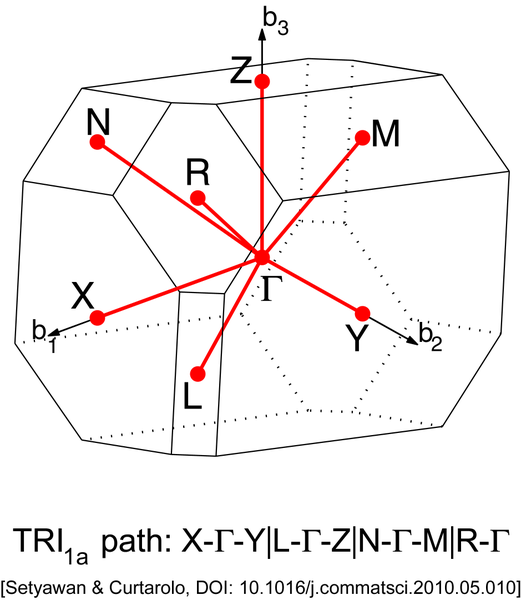
\includegraphics[width=0.2\linewidth,clip=true]{Figs/Brillouinzones/521px-TRI1a.PNG}
%% 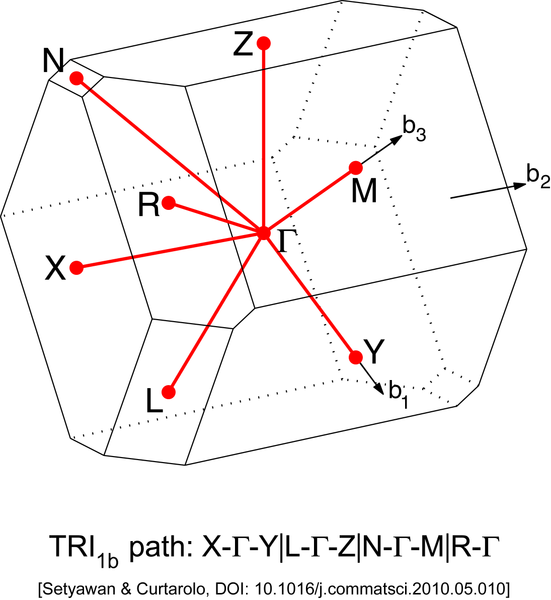
\includegraphics[width=0.2\linewidth,clip=true]{Figs/Brillouinzones/551px-TRI1b.PNG}
%% 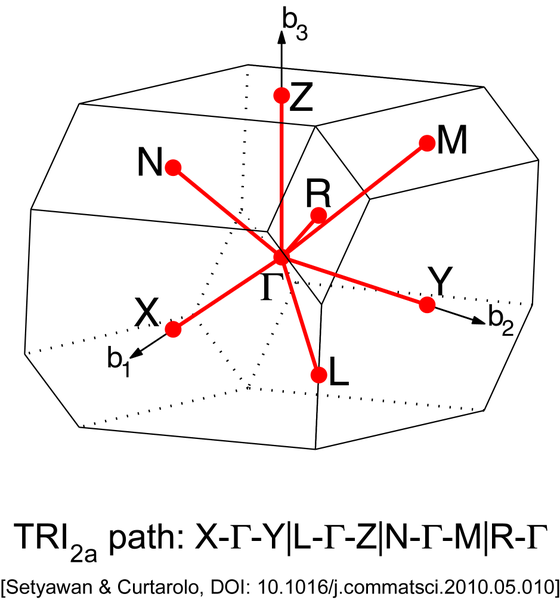
\includegraphics[width=0.2\linewidth,clip=true]{Figs/Brillouinzones/560px-TRI2a.PNG}

%% 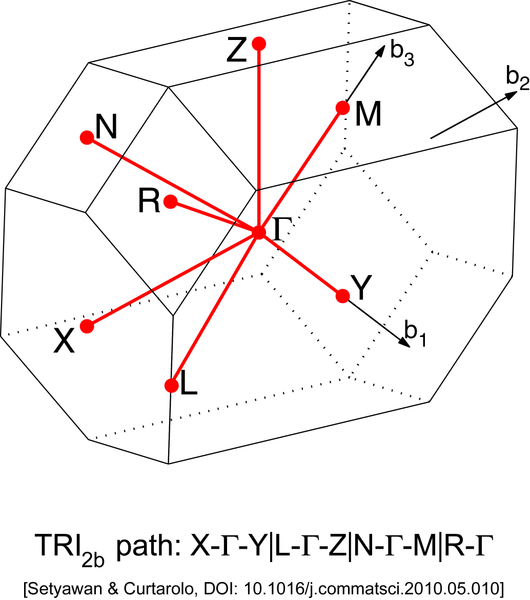
\includegraphics[width=0.2\linewidth,clip=true]{Figs/Brillouinzones/530px-TRI2b.PNG}

%% %=======================================================
%% \subsection{Monoclinic lattice system}
%% %=======================================================
%% 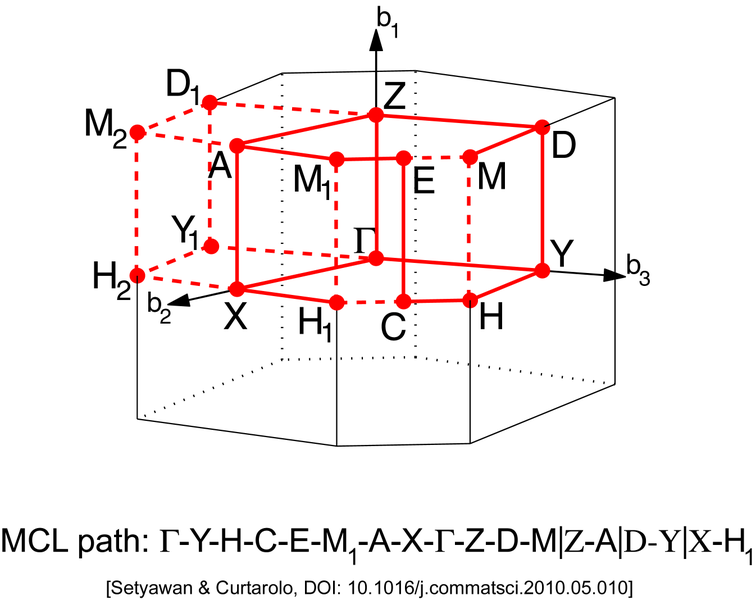
\includegraphics[width=0.2\linewidth,clip=true]{Figs/Brillouinzones/756px-MCL.PNG}
%% 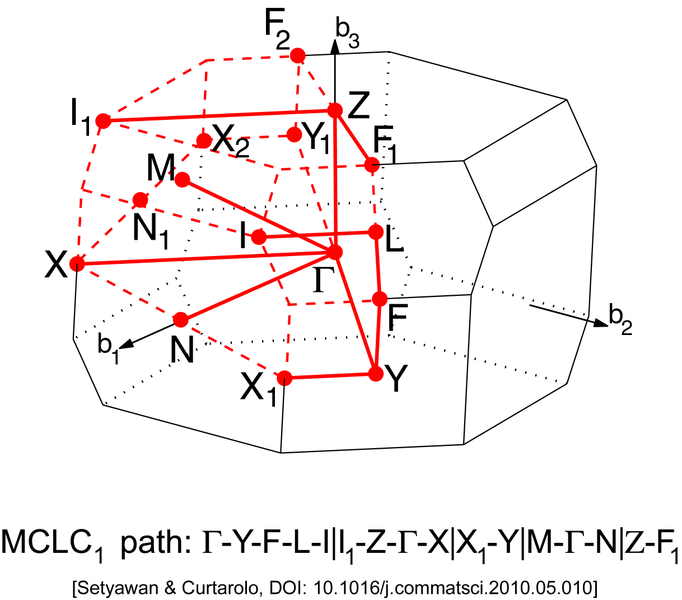
\includegraphics[width=0.2\linewidth,clip=true]{Figs/Brillouinzones/682px-MCLC1.PNG}
%% 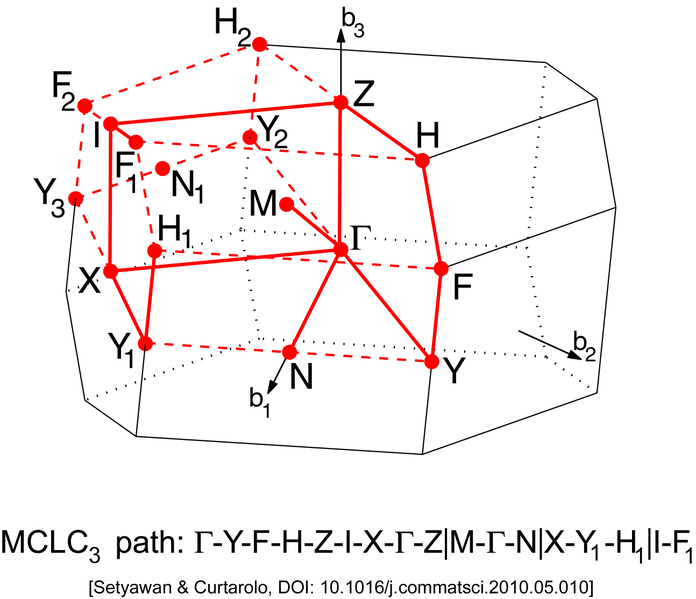
\includegraphics[width=0.2\linewidth,clip=true]{Figs/Brillouinzones/696px-MCLC3.PNG}

%% 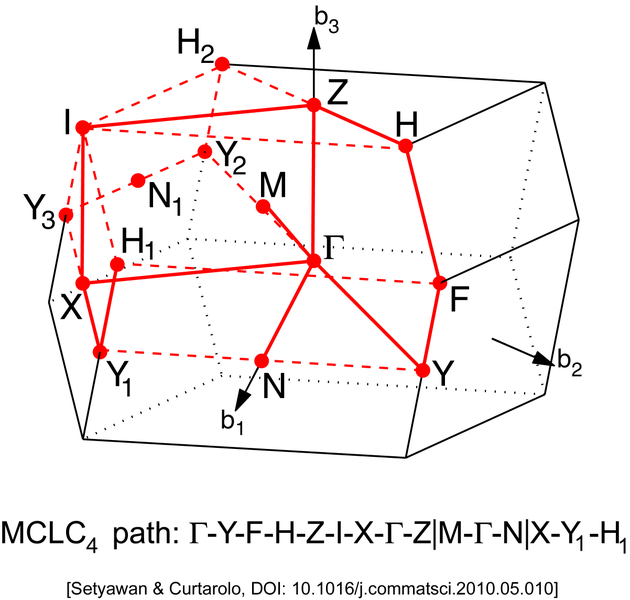
\includegraphics[width=0.2\linewidth,clip=true]{Figs/Brillouinzones/630px-MCLC4.PNG}
%% 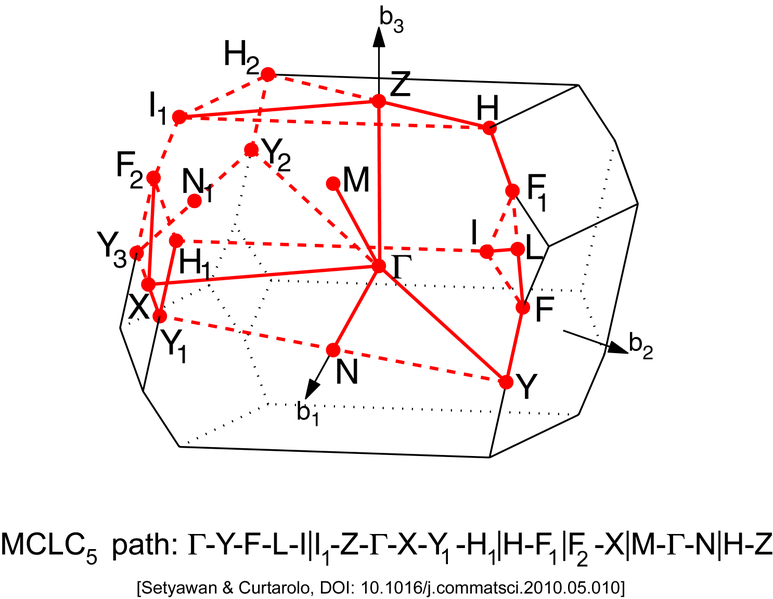
\includegraphics[width=0.2\linewidth,clip=true]{Figs/Brillouinzones/773px-MCLC5.PNG}

%% %=======================================================
%% \subsection{Orthorhombic lattice system}
%% %=======================================================
%% 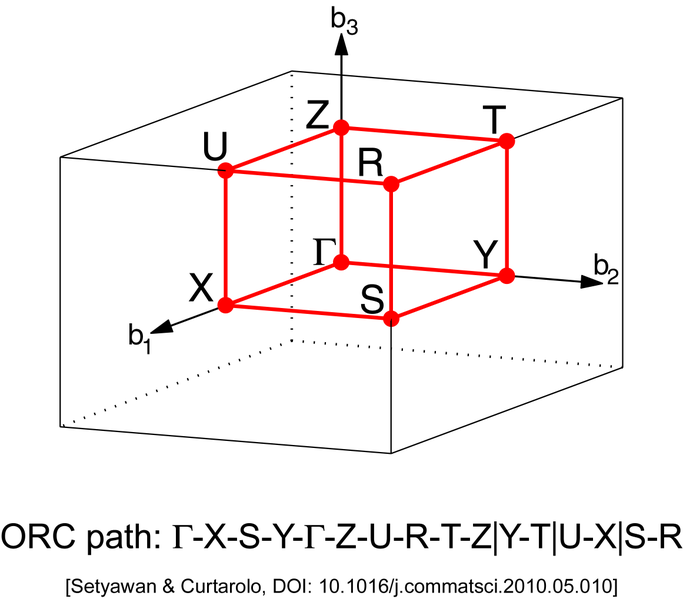
\includegraphics[width=0.2\linewidth,clip=true]{Figs/Brillouinzones/656px-ORCF3.PNG
%% \includegraphics[width=0.2\linewidth,clip=true]{Figs/Brillouinzones/683px-ORC.PNG}
%% 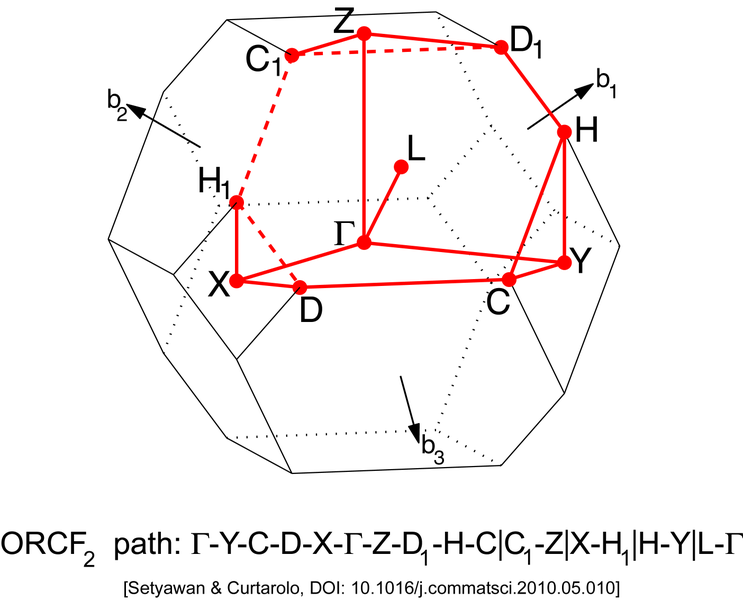
\includegraphics[width=0.2\linewidth,clip=true]{Figs/Brillouinzones/743px-ORCF2.PNG}

%% 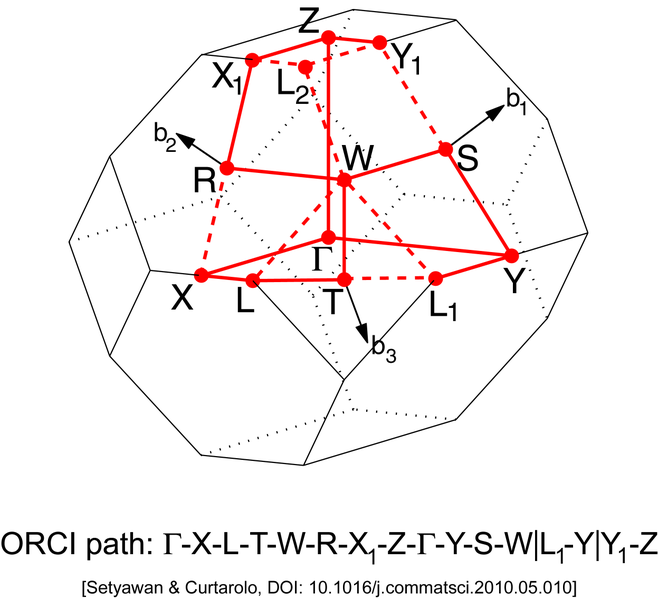
\includegraphics[width=0.2\linewidth,clip=true]{Figs/Brillouinzones/658px-ORCI.PNG}
%% 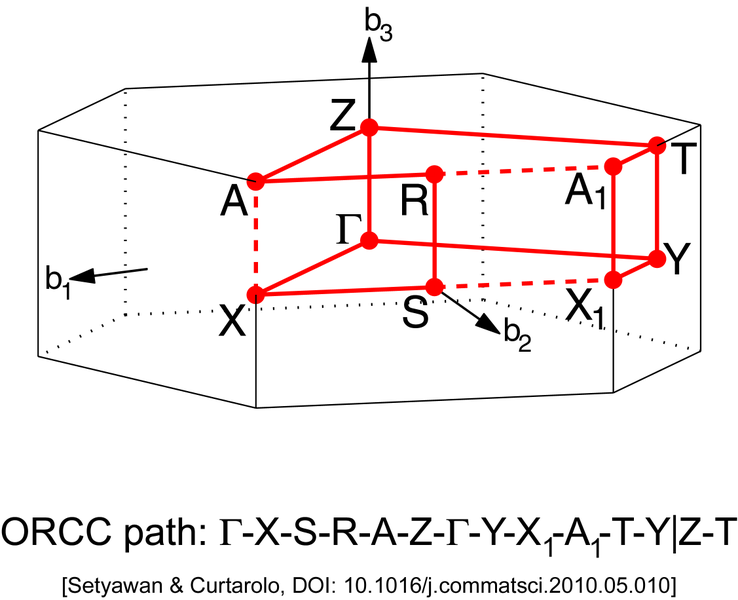
\includegraphics[width=0.2\linewidth,clip=true]{Figs/Brillouinzones/738px-ORCC.PNG}
%% 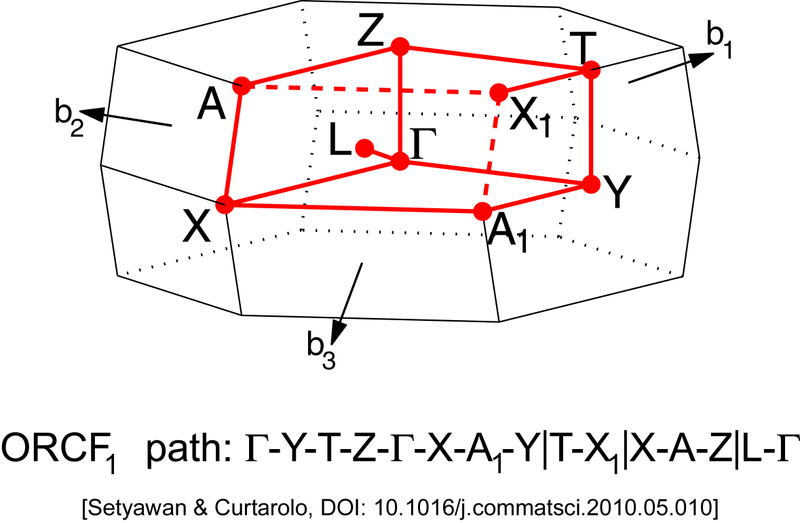
\includegraphics[width=0.2\linewidth,clip=true]{Figs/Brillouinzones/800px-ORCF1.PNG}

%% %=======================================================
%% \subsection{Tetragonal lattice system}
%% %=======================================================
%% 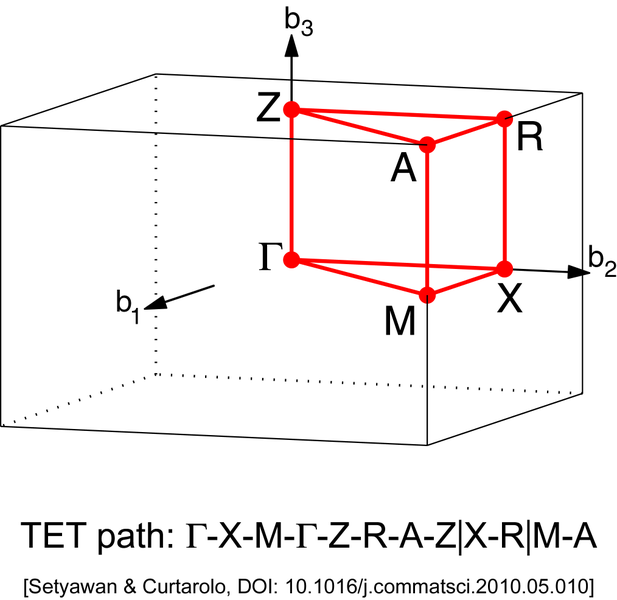
\includegraphics[width=0.2\linewidth,clip=true]{Figs/Brillouinzones/617px-TET.PNG}
%% 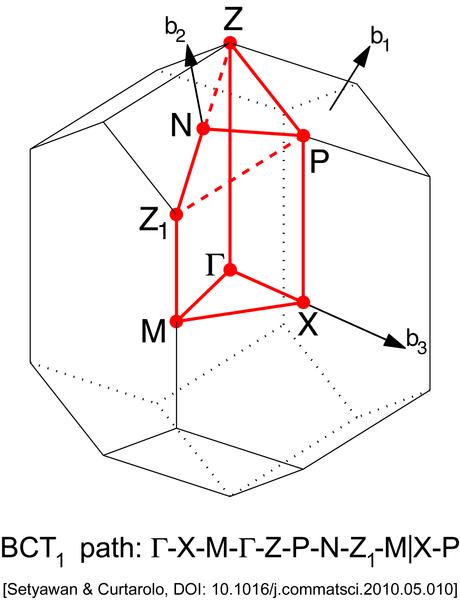
\includegraphics[width=0.2\linewidth,clip=true]{Figs/Brillouinzones/460px-BCT1.PNG}
%% 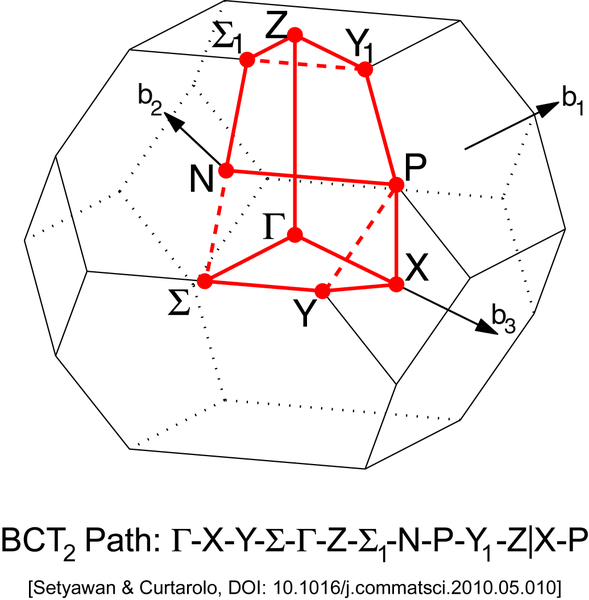
\includegraphics[width=0.2\linewidth,clip=true]{Figs/Brillouinzones/589px-BCT2.PNG}

%% %=======================================================
%% \subsection{Rhombohedral lattice system}
%% %=======================================================
%% 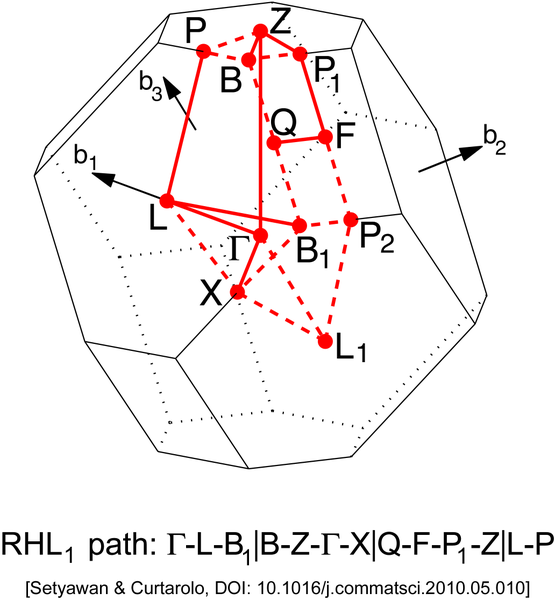
\includegraphics[width=0.2\linewidth,clip=true]{Figs/Brillouinzones/555px-RHL1.PNG}
%% 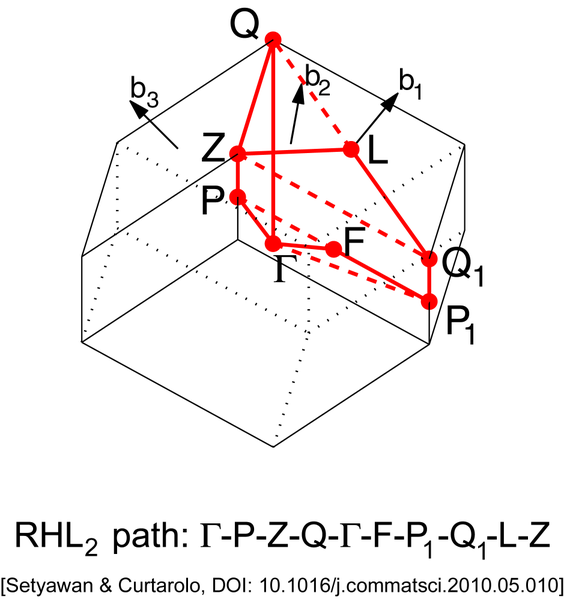
\includegraphics[width=0.2\linewidth,clip=true]{Figs/Brillouinzones/564px-RHL2.PNG}

%% %=======================================================
%% \subsection{Hexagonal lattice system}
%% %=======================================================
%% 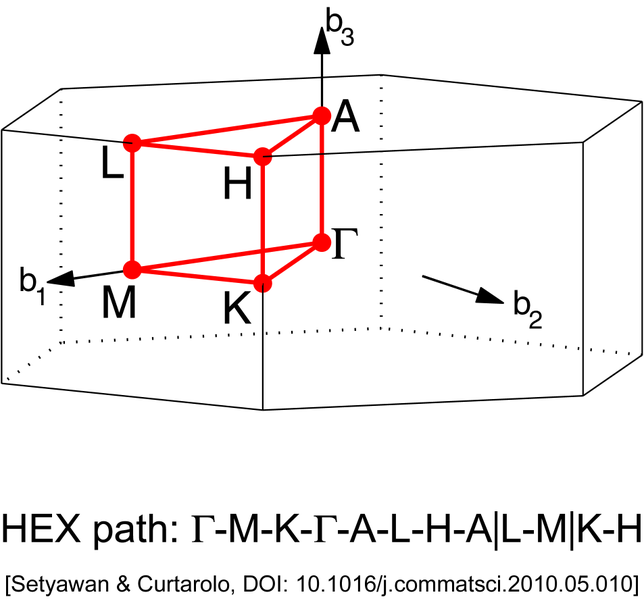
\includegraphics[width=0.2\linewidth,clip=true]{Figs/Brillouinzones/644px-Brillouin_zone_in_hexagonal_lattice.png}

%% %=======================================================
%% \subsection{Cubic lattice system}
%% %=======================================================
%% 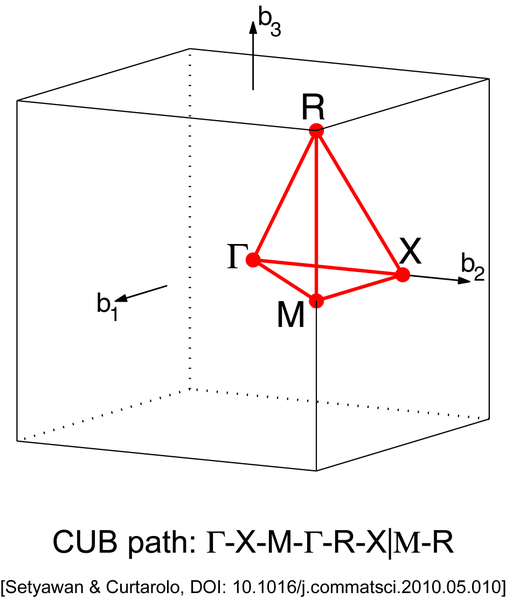
\includegraphics[width=0.2\linewidth,clip=true]{Figs/Brillouinzones/506px-CUB.PNG}
%% 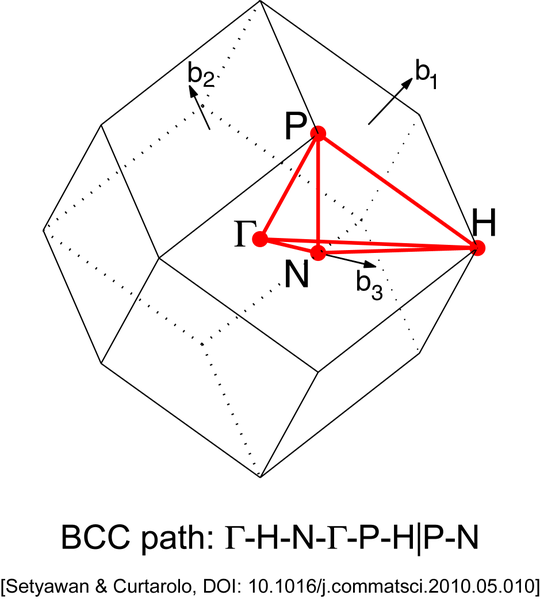
\includegraphics[width=0.2\linewidth,clip=true]{Figs/Brillouinzones/540px-BCC.PNG}
%% 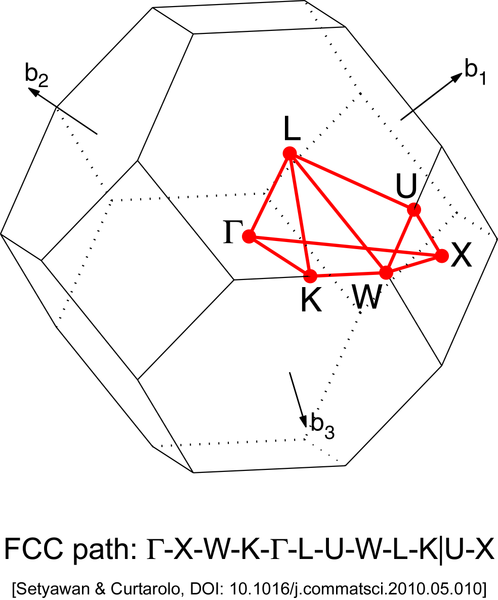
\includegraphics[width=0.2\linewidth,clip=true]{Figs/Brillouinzones/498px-FCC.PNG}

\clearpage

\bibliographystyle{unsrtnat}
\bibliography{../all}
\end{document}  
